\documentclass{beamer}
\usetheme{metropolis}           % Use metropolis theme
\usecolortheme{beaver}
\setbeamerfont{caption}{size=\scriptsize}
\title{Programación Evolutiva}
\subtitle{Resolución de nonogramas mediante métodos evolutivos}
\date{2022-2023}
\author{Alejandro Barrachina Argudo \\ Adrià Carreras Bagur}
\institute{Universidad Complutense de Madrid}
\begin{document}
\maketitle

\begin{frame}{Tabla de contenidos}
    \tableofcontents
\end{frame}

\AtBeginSection[]{
    \begin{frame}{Tabla de contenidos}
        \tableofcontents[currentsection]
    \end{frame}
}
\AtBeginSubsection[]{
    \begin{frame}{Tabla de contenidos}
        \tableofcontents[currentsubsection]
    \end{frame}
}
\section{Introducción}
\begin{frame}{Introducción}

    Los \textit{nonogramas} son puzzles que consisten en colorear celdas de un tablero según una serie de restricciones para formar imágenes.

    \begin{figure}
        \centering
        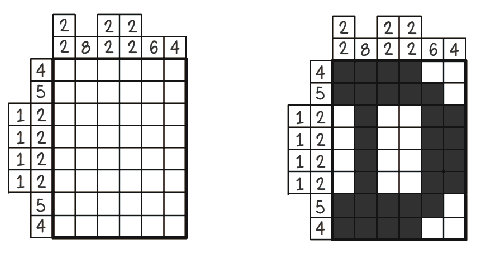
\includegraphics[width=4cm]{Images/nonograma.png}
        \caption{ Nonograma antes de su resolución (izquierda) y tras su resolución}
    \end{figure}

\end{frame}
\section{Nonogramas en programación evolutiva}
\begin{frame}
    \frametitle{Esquema evolutivo}

    Para poder resolver este problema de forma evolutiva usaremos la siguiente representación:
    \begin{itemize}
        \item <1-> El tablero se representará como una matriz de booleanos, marcando si la casilla está coloreada o no
        \item <2-> Dos listas de enteros con las restricciones de filas y columnas, cada posición de las listas será una lista de restricciones de esa fila/columna
    \end{itemize}

\end{frame}
\subsection{Fitness}

\begin{frame}
    \frametitle{Fitness}

    Para calcular el fintess aplicaremos la siguiente función sobre cada fila y cada columna:
    \begin{enumerate}
        \item <1-> Se cogen las restricciones de la fila/columna
        \item <2-> Se cuentan los conjuntos de casillas marcadas seguidas y el número de casillas marcadas totales
        \item <3-> Si el número de conjuntos es el mismo número o menor que el total de restricciones, se proporciona una recompensa, en caso contrario se aplica una penalización
        \item <4-> Si el número de casillas marcadas de un conjunto cumple con su restricción se da una recompensa, si hay más casillas seguidas que en las restricciones se penaliza con el exceso
        \item <5-> En caso de que el número de casillas marcadas sea igual que el número final de casillas marcadas según las restricciones, consigue una recompensa
    \end{enumerate}
\end{frame}
\subsection{Cruces}
\begin{frame}
    \frametitle{Cruces}
    Hemos hecho pruebas con cuatro tipos de cruce de dos individuos:
    \begin{itemize}
        \item <1-> Uniforme: hay un 50\% de posibilidades de intercambiar una casilla de ambos individuos
        \item <2-> Monopunto: se intercambian todas las casillas de ambos individuos a partir de un punto aleatorio. Solo afecta a las filas
        \item <3-> XOR: uno de los dos individuos seleccionado aleatoriamente se queda como descendiente directo, el otro descendiente se forma a partir de hacer la operación XOR a los tableros de ambos individuos
        \item <4-> ColFil: crea un descendiente con las mejores filas de cada individuo y otro con las mejores columnas de cada individuo
    \end{itemize}
\end{frame}
\subsection{Mutaciones}
\begin{frame}
    \frametitle{Mutaciones}
    Usamos cuatro tipos de mutaciones:
    \begin{itemize}
        \item <1-> Básica: cada casilla tiene un 50\% de cambiar de estado
        \item <2-> Inversión: invierte el cromosoma entre dos puntos escogidos aleatoriamente
        \item <3-> Heurística: como la básica, pero si el cambio empeora el fitness lo revierte
        \item <4-> Rotación heurística: rota posiciones del cromosoma siempre y cuando tengan mejor fitness
    \end{itemize}
\end{frame}
\subsection{Otros mecanismos}
\begin{frame}
    \frametitle{Otros mecanismos}
    Para facilitar la introducción de datos y la resolución de los nonogramas proporcionados se implementan dos mecanismos propios de esta práctica:
    \begin{itemize}
        \item <1-> Introducción de archivos: un archivo en texto plano que contiene la siguiente estructura:
              \begin{itemize}
                  \item <1-> Primera línea con el número de filas
                  \item <1-> N lineas con las restricciones de cada fila
                  \item <1-> Línea con el número de columnas
                  \item <1-> N líneas con las restricciones de cada columna
              \end{itemize}
        \item <2-> Prevención de estancamiento de la población mediante reinicio de población: si la población tiene una media similar durante dos generaciones seguidas o se aproxima demasiado al mejor individuo de todas las generaciones, reiniciamos la población quedándonos solo con la élite
    \end{itemize}
\end{frame}

\section{Pruebas de concepto}
\subsection{5x5}
\begin{frame}
    \frametitle{5x5}
    \begin{figure}
        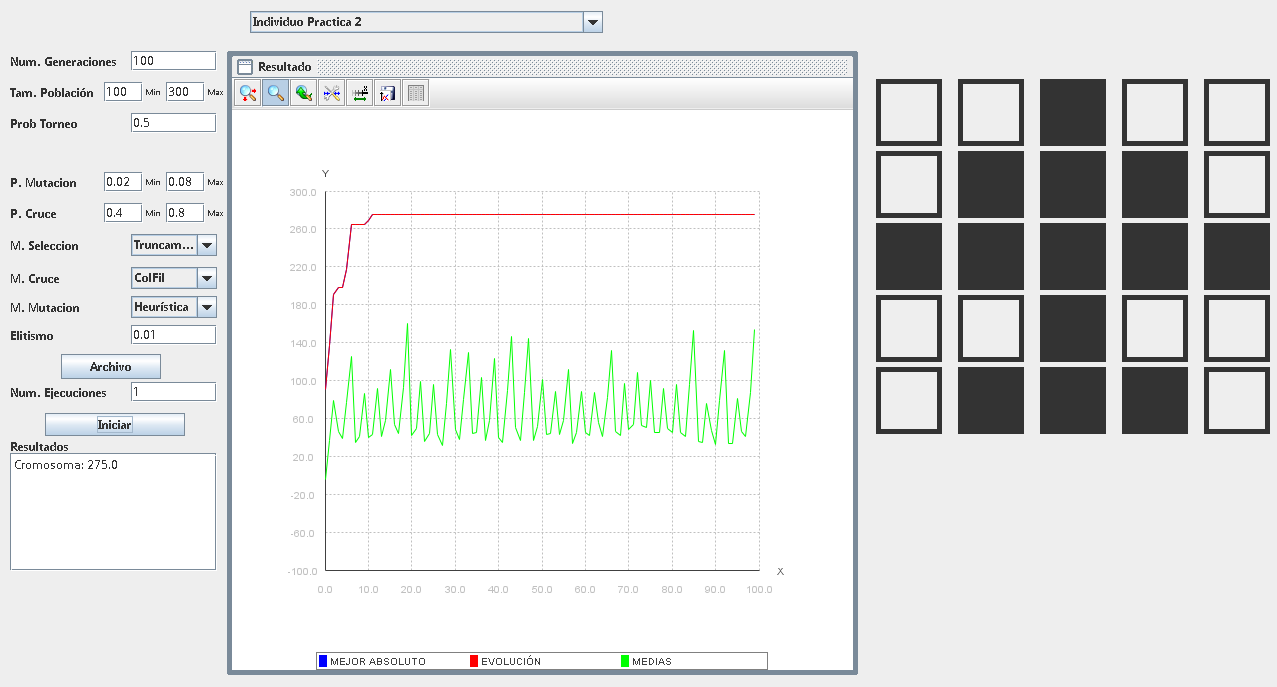
\includegraphics[width=\textwidth]{Images/5x5.png}
        \caption{Nonograma 5x5: pica}
    \end{figure}
\end{frame}
\subsection{10x10}
\begin{frame}
    \frametitle{10x10}
    \begin{figure}
        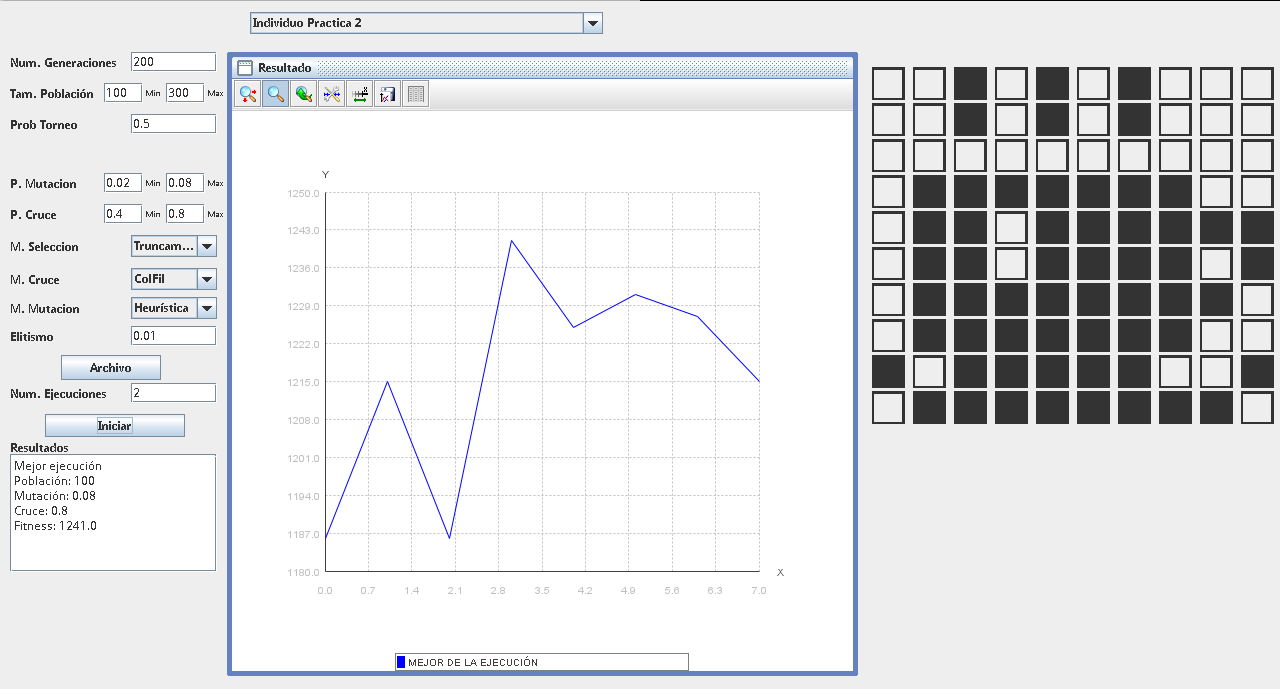
\includegraphics[width=\textwidth]{Images/10x10.png}
        \caption{Nonograma 10x10: taza de café}
    \end{figure}
\end{frame}
\subsection{15x15}
\begin{frame}
    \frametitle{15x15}
    \begin{figure}
        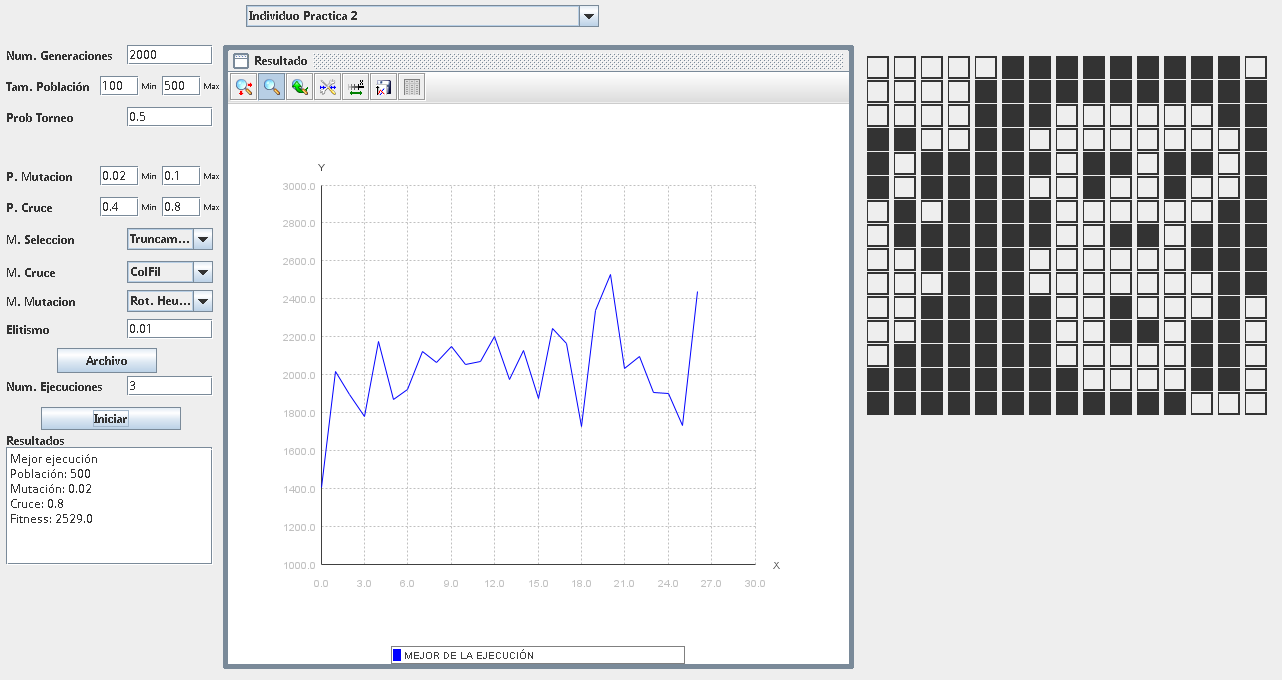
\includegraphics[width=\textwidth]{Images/15x15.png}
        \caption{Nonograma 15x15: cara de mono}
    \end{figure}
\end{frame}

\section{Observaciones}
\begin{frame}
    \frametitle{Observaciones}
    Se tuvo que implementar un sistema de reinicio de población ya que al ser problemas muy complejos (10x10 y 15x15) se alcanzaban máximos locales y se quedaba estancada la población
\end{frame}
\begin{frame}
    \frametitle{Observaciones}
    Los mejores resultados se obtuvieron con Truncamientos como método de selección, ColFil como método de cruce y cualquiera de los métodos heurísticos de mutación. Sin ellos, el problema es lo suficientemente complejo como para que no encuentre soluciones completas
\end{frame}

\section{Conclusiones}
\begin{frame}
    \frametitle{Conclusiones}
    Resolver nonogramas de forma evolutiva no es nada nuevo en este campo, hay estudios generando estrategias óptimas de resolución, comparando este método frente a búsquedas de soluciones en árboles y grafos, etc.
    Aún no siendo algo innovador, si ha sido interesante crear métodos propios de cruce y mutación para llegar a soluciones óptimas, así como encontrar un fitness adecuado para no sobrecompensar ninguna acción.
\end{frame}
\end{document}
